\begin{figure}[H]
    \begin{subfigure}[t]{.2\textwidth}
        \caption{}
        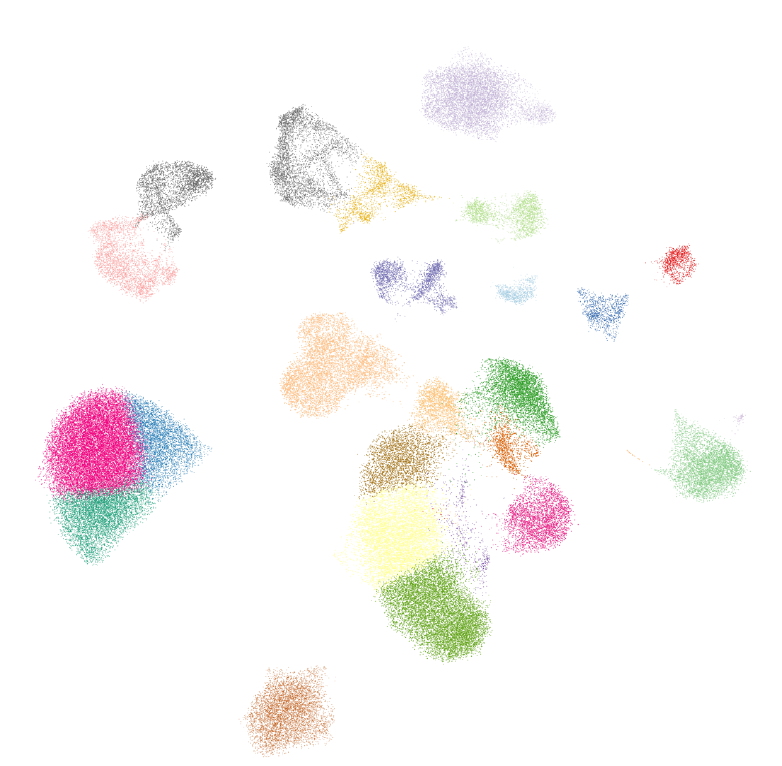
\includegraphics[width=\textwidth]{./extended_plots/cell_proj_with_leiden.png}        
    \end{subfigure}
    \begin{subfigure}[t]{.2\textwidth}
        \caption{}
        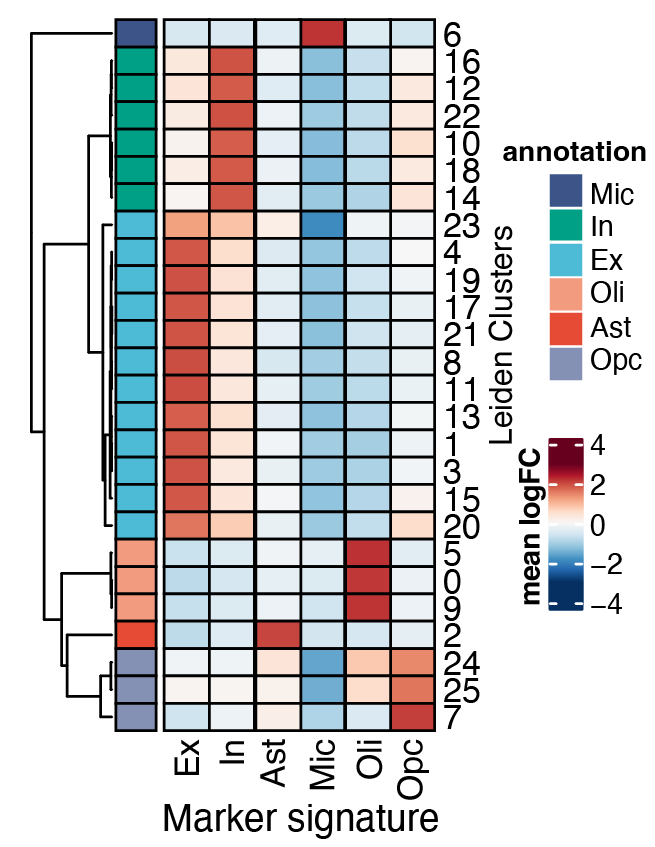
\includegraphics[width=\textwidth]{./extended_plots/leiden_heatmap.png}        
    \end{subfigure}   
    \begin{subfigure}[t]{.15\textwidth}
        \caption{}
        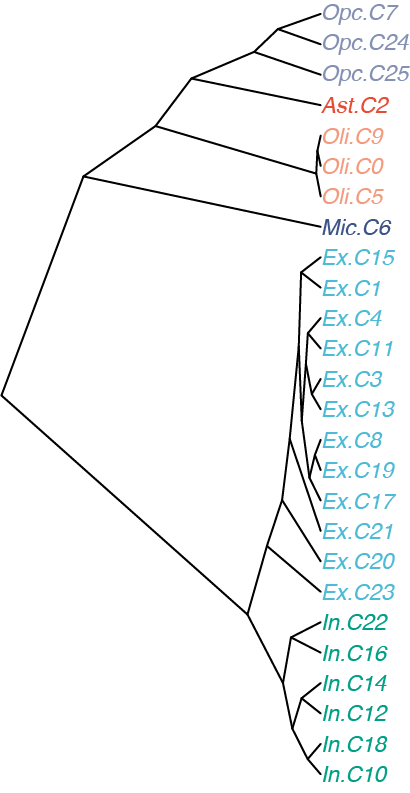
\includegraphics[width=\textwidth]{./extended_plots/hierarchical_tree.png}        
    \end{subfigure}           
    \begin{subfigure}[t]{.15\textwidth}
        \caption{}
        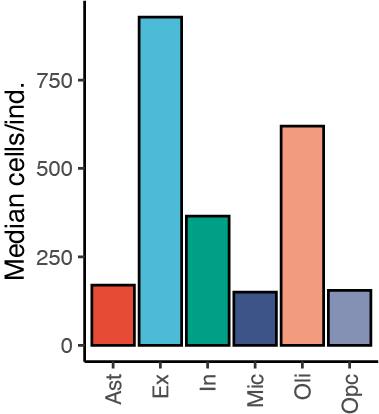
\includegraphics[width=\textwidth]{./extended_plots/median_cells.png}        
    \end{subfigure}       
    \begin{subfigure}[t]{.2\textwidth}
        \caption{}
        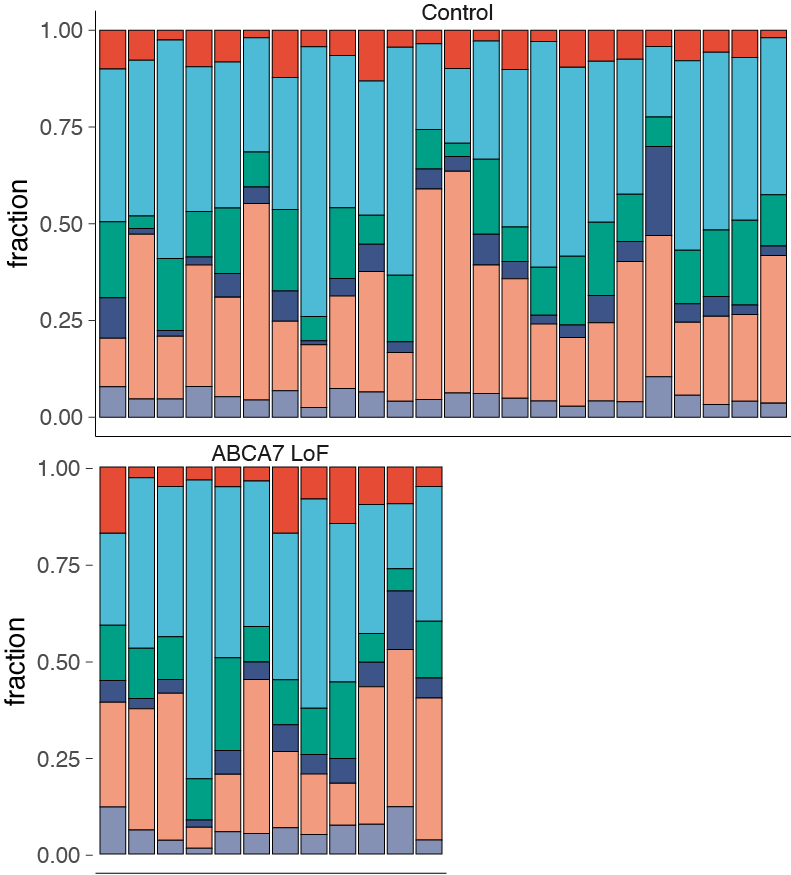
\includegraphics[width=\textwidth]{./extended_plots/individual_fractions.png}        
    \end{subfigure}     
    \begin{subfigure}[t]{.25\textwidth}
        \caption{}
        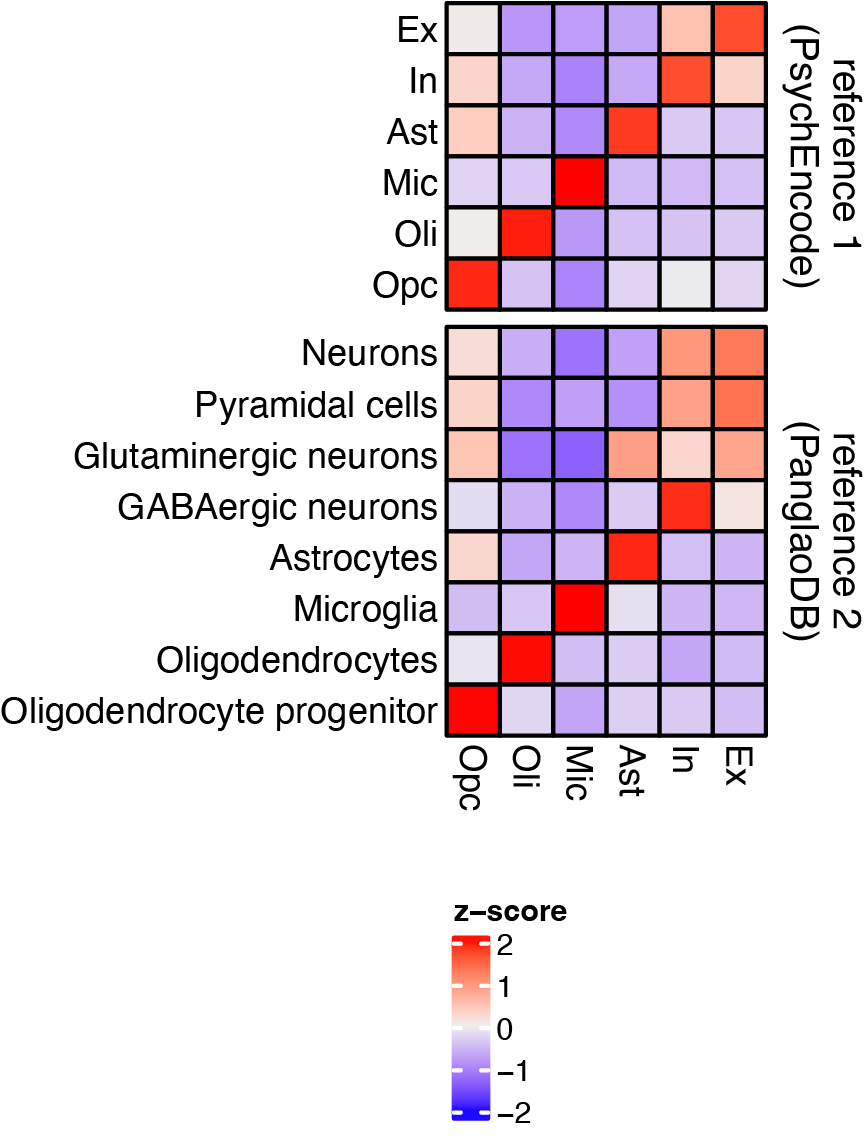
\includegraphics[width=\textwidth]{./extended_plots/marker_hmap.png}        
    \end{subfigure}         
    \begin{subfigure}[t]{.2\textwidth}
        \caption{}
        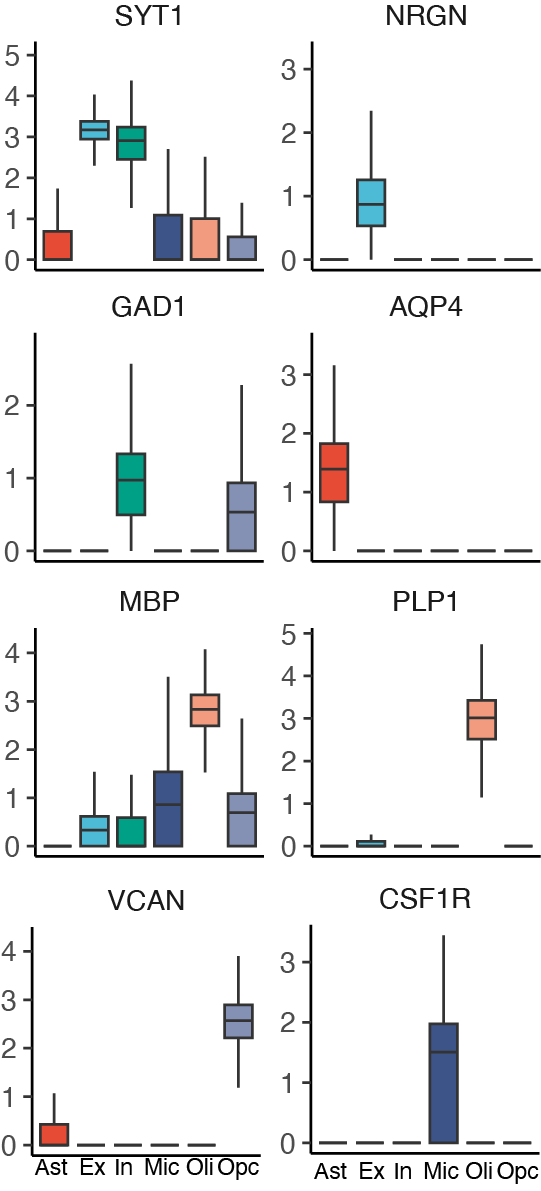
\includegraphics[width=\textwidth]{./extended_plots/marker_boxplot.png}        
    \end{subfigure}       
    \begin{subfigure}[t]{.25\textwidth}
        \caption{}
        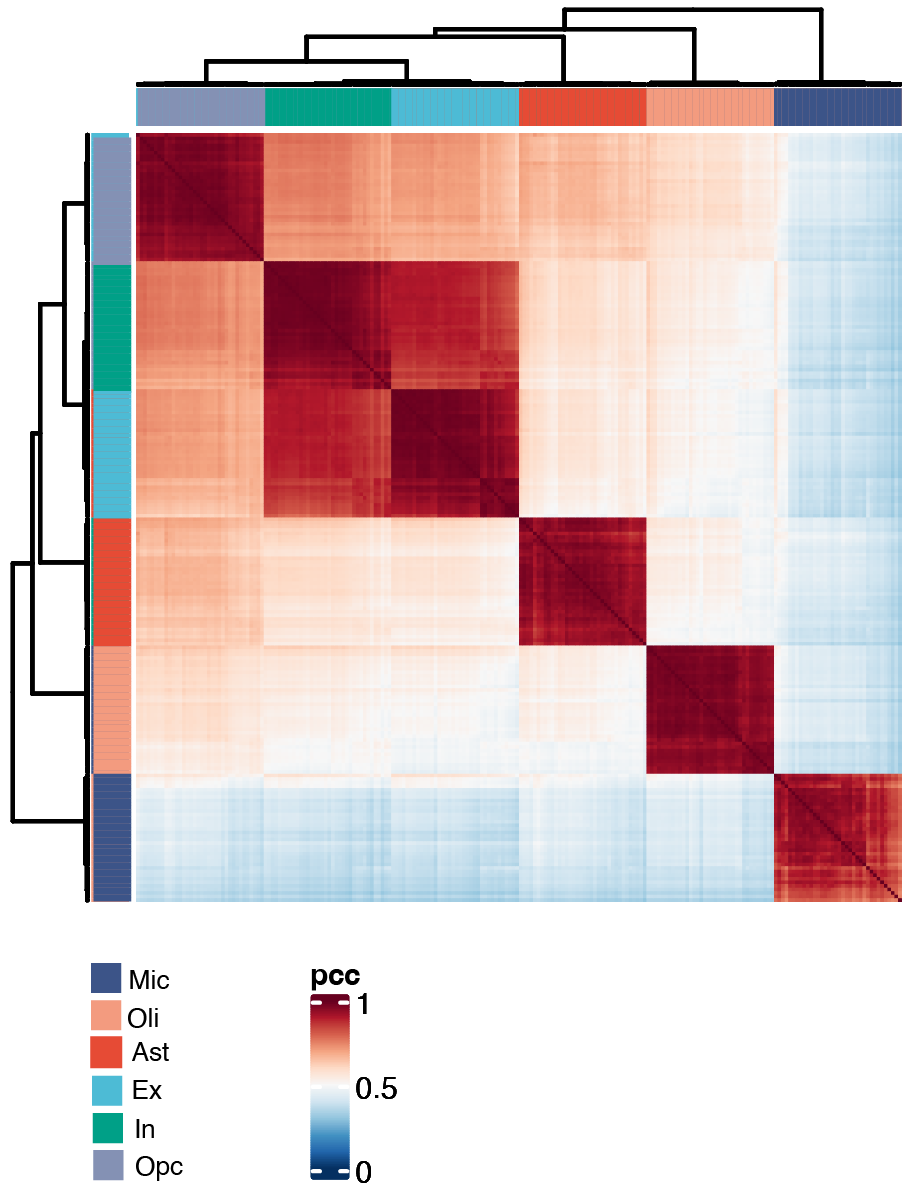
\includegraphics[width=\textwidth]{./extended_plots/celltype_heatmap.png}        
    \end{subfigure}       
    \begin{subfigure}[t]{.2\textwidth}
        \caption{}
        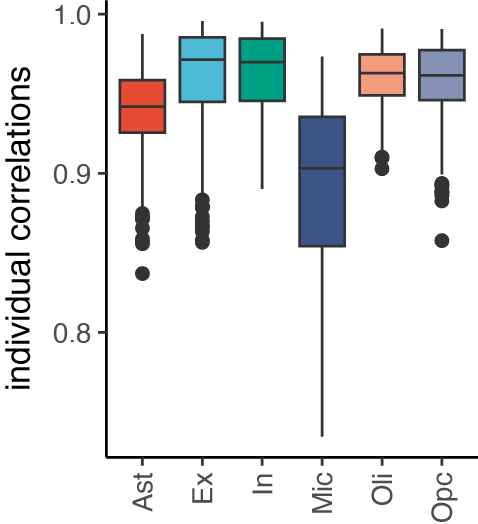
\includegraphics[width=\textwidth]{./extended_plots/individual_correlations.png}        
    \end{subfigure}       
    \caption{
        \textbf{Overview of snRNA-sequencing Batch Correction, Data Quality, and Cell Type Annotations.}\\
    }
    \label{fig:snRNA_quality_annotation}
\end{figure}
\begin{itemize}
    \item[\textbf{(A)}] Two-dimensional UMAP projections of individual cells from gene expression space, colored by Leiden clusters. 
    \item[\textbf{(B)}] Average marker gene expression (per-cluster mean log(fold-change)) for all marker genes for the cell type indicated along the x-axis. Log(fold-changes) are computed for the cluster of interest vs. all remaining clusters. Reference 1 (Table 2) marker genes were used. 
    \item[\textbf{(C)}] Cladogram visualizing subcluster relationships based on pairwise distances between per-cluster gene expression profiles. 
    \item[\textbf{(D)}] Average marker gene expression profiles (x-axis) per major cell type annotation (y-axis) for two marker gene references (Table 2). 
    \item[\textbf{(E)}] Per-cell distribution of select marker gene expression by cell type. Y-axis indicates log counts. 
    \item[\textbf{(F)}] Median number of cells per cell type per individual. 
    \item[\textbf{(G)}] Cell type fraction by individual. 
    \item[\textbf{(H,I)}] Individual-level gene expression correlations by cell type. 
\end{itemize}
For all panels, p-values for all continuous variables were computed by two-sided Wilcoxon rank sum test. 
P-values for all discrete variables were computed by two-sided Fisher’s exact test. 
For A, I, M boxes indicate per-condition dataset quartiles, and whiskers extend to the most extreme data points not considered outliers (i.e., within 1.5 times the interquartile range from the first or third quartile).